\section{Instrução para execução}
	Basta mudar rodar o código. Por padrão, o grafo deve estar em um arquivo nomeado ``grafo.txt", no mesmo diretório. 

	Caso queria testar um grafo descrito com outro nome de arquivo, basta mudar no código.  

\section{Entrada utilizada}
	A entrada dada em sala. Pode ser encontrada no arquivo ``grafo.txt", no GitHub. 

	\begin{table}[h!]
		\centering
		\begin{tabular}{ccc}
			\hline
			$v_i$ & $v_j$ & $peso_{ij}$ \\
			\hline
			1 & 2 & 7 \\
			1 & 3 & 5 \\
			2 & 4 & 9 \\
			3 & 5 & 6 \\
			4 & 5 & 0 \\
			4 & 6 & 11 \\
			5 & 7 & 4 \\
			6 & 8 & 3 \\
			7 & 8 & 8 \\
			8 & 9 & 6 \\
			8 & 10 & 4 \\
			10 & 9 & 0 \\
			9 & 11 & 7 \\
			\hline
		\end{tabular}
	\end{table}

	\section{Saída obtida}
	Está de acordo com o esperado. nenhuma inconsistÊncia observada. 

	\begin{figure}[h!]
		\centering

		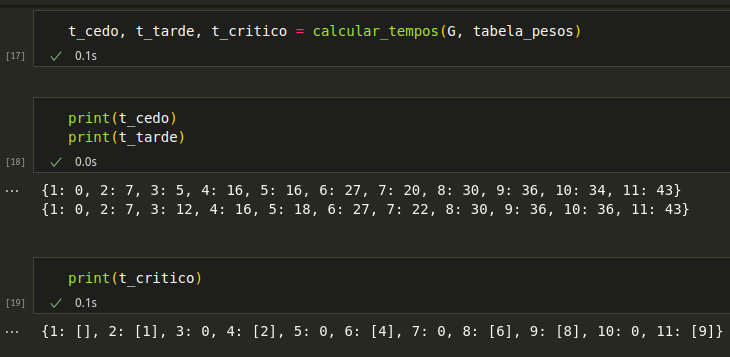
\includegraphics[width = 10cm]{resultado.png}
		\caption{Resultado}
	\end{figure}

\newpage


\section{Código}
O código encontra-se disponível no seguinte repositório: 
\href{https://github.com/RodrigoZonzin/grafos}{https://github.com/RodrigoZonzin/grafos}. Também está no portal.